\subsection{Segregation of duties}

Questo concetto è molto importante.

La \textit{conformità} è più importante della \textit{sicurezza} perché 
bisogna essere conformi a degli standard.

È importante, come già detto in precedenza, separare i vari 
poteri tra le persone, in maniera tale da assicurarsi che non avvengano 
``abusi di potere'' (es. l'amministratore di rete concede i diritti, ma 
qualcuno deve autorizzare che il ruolo $x$ necessiti dei diritti. 
l'amministratore implementa la concessione). 

È importante anche che gli \textit{asset} vengano controllati. Solitamente gli 
\textit{asset} sono fisici, ma nel settore IT possono essere immateriali (come 
un file contente un disegno di un progetto per una architettura di rete). 
Quindi è importante documentare le responsabilità. Si è responsabili quando 
occorrono \textit{due condizioni:} quando si è nominati ufficialmente (tramite 
una delega formale) o quando si hanno i poteri per implementare correttamente 
quanto richiesto.

\subsubsection{Personale}

Dal punto di vista della sicurezza il personale è sempre l'anello debole. 
Il \textit{background check} dipende sempre in base alla mansione che 
dev'essere coperta. Questi controlli sono abbastanza sensibili.
Se viene maneggiato denaro o \textit{asset} sicuramente è necessario eseguire 
un \textit{background check} per assicurarsi la \textit{professionalità} e 
l'\textit{affidabilità} della persona (anche essere coinvolti in una stupida 
rissa potrebbe compromettere l'affidabilità di una persona). Di conseguenza, i 
propri profili social dovrebbero essere sempre controllati in maniera tale da 
non contenere contenuto non appropriato.

Il \textit{monitoring} delle email è un problema ovunque, tranne negli USA: 
lì le email non sono protette. L'azienda fa lo scan dei PC dei 
dipendenti. In Italia, dopo un caso eclatante, la giurisprudenza permette di 
leggere le email di lavoro.

\paragraph{Assunzione degli impiegati}

Bisogna fare attenzione quando si eseguono assunzioni: è 
importante anche controllare che chi viene assunto non esegua manomissioni dei 
documenti ufficiali\footnote{La falsificazione di documenti nella pubblica 
amministrazione comporta una reclusione dai 2 ai 5 anni.} (es. dichiarate di 
essere laureato senza una laurea).

Il \textbf{mansionario} specifica cosa un impiegato deve fare.

\textbf{Confidentiality agreement}: contratto in cui il lavoratore dichiara di 
non divulgare nulla di quello su cui lavora l'azienda e indica anche un limite 
di tempo per cui l'impiegato non può svolgere un lavoro nello stesso campo.


\paragraph{Orientamento dei nuovi impiegati}

Quando un nuovo impiegato firma un documento ha letto e accettato le policy di 
sicurezza. Inoltre si impegna a:
\begin{itemize}
\item non divulgare ID e password per il login;
\item creare password di qualità;
\item bloccare il terminale quando non è presente;
\item riportare violazioni della sicurezza sospette;
\item mantenere una buona sicurezza fisica.
\end{itemize}

\paragraph{Employee termination}

Quando si arriva al termine del periodo lavorativo si deve ritornare 
l'equipaggiamento aziendale e revocare l'accesso all'individuo. Badge e 
cartellini devono essere riconsegnati; le autorizzazioni che l'individuo aveva 
all'interno dell'azienda devono essere revocate.

\subsubsection{Accordi tra terze parti}

Definiscono le \textit{policy} di sicurezza relative alle informazioni e le 
procedure per implementare le \textit{policy}; forniscono controlli per 
proteggersi contro software malevolo. Pubblicano restrizioni per la copia e la 
distribuzione delle informazioni, implementano procedure per determinare se 
gli \textit{asset} sono stati compromessi e assicurano il ritorno o la 
distruzione dei dati al termine del rapporto lavorativo.

\subsubsection{Riassunto dei controlli sul personale}

I punti importanti del controllo sul personale sono:
\begin{itemize}
\item Segregation of Duties;
\item Vacanze obbligatorie e rotazione delle mansioni;
\item Addestramento delle policy e procedure;
\item Controlli del background;
\item Need to know/Least privilege;
\item Meccanismo di segnalazione di frodi.
\end{itemize}

\section{Esercizi}

Gli esercizi sono disponibili nella parte \ref{esSFDP:generali}

\part{Security Management}
\label{SM}

\paragraph{Obiettivi}

Gli obiettivi di questa parte del corso sono:
\begin{itemize}
\item Quality assurance;
\item Capire i ruoli di CISO, CIO, CSO Board of directors, Executive 
Management, ecc;
\item Definire delle baseline sulla sicurezza ;
\item Descrivere COBIT, CMM (vecchio), livelli 1-5.
\end{itemize}

\chapter{COBIT, CMM}

\section{CMM}
\textbf{CMM} sta per \textit{Capability Maturity Model}. Si è capito che lo 
sviluppo del software è cruciale nelle società che lo sviluppano, le quali 
vengono mappate in 5 livelli dove ogni livello identifica la maturità di 
un'azienda.
I cinque livelli sono:
\begin{enumerate}
  \item \textbf{Initial:} si ``vive alla giornata''. Si è estremamente 
  reattivi agli eventi che accadono e non è in atto alcun tipo di 
  pianificazione/processo;
  \item \textbf{Managed:} si ha ancora un approccio di tipo reattivo agli 
  eventi che accadono, ma si comincia ad definire processi ed ad avere 
  pianificazioni per i progetti;
  \item \textbf{Defined:} si cominciano a definire processi anche per 
  l'organizzazione in toto e si comincia ad avere un approccio proattivo ai 
  problemi;
  \item \textbf{Qualitatively Managed:} vengono applicate misurazioni e
  metriche ai processi per poter controllarli e migliorarli continuamente;
  \item \textbf{Optimized:} una volta che è in atto il miglioramento continuo 
  dei processi che vengono a loro volta misurati tramite metriche l'azienda 
  può puntare ad ottimizzarli il più possibile.
\end{enumerate}
Il CMM è stato superato dal CMMI \textit{Capability Maturity Model Integration}


Il \textbf{COBIT} è uno standard diverso.


\subsection{Livello 0}

Al livello iniziale si è come un pompiere: si corre continuamente a destra e a 
sinistra per risolvere eventuali problemi.

\subsection{Livello 1 - Esecuzione informale}

La progettazione della sicurezza è definita in maniera povera, i problemi di 
sicurezza sono trattati in maniera reattiva: si reagisce 
alla minaccia, portando prima o poi l'attacco a vincere. Non ci sono piani di 
contingenza\footnote{I piani di contingenza sono dei piani che dettano le 
azioni da compiere in caso si verificano delle situazioni d'emergenza.}. I 
budget, la qualità, le funzionalità e i progetti vengono schedulati \textit{ad 
hoc}. Non ci sono aree dei processi.

\subsection{Livello 2 - Pianificato e Tracciato}

Le procedure vengono definite a livello di progetto. La definizione, 
pianificazione e le performance diventano de-facto standard da progetto a 
progetto. Gli eventi vengono tracciati. Le funzionalità comuni includono: 
pianificazione, disciplina, verifica e tracciamento delle performance.

\subsection{Livello 3 - Ben definito}

I processi di sicurezza sono standardizzati all'interno dell'organizzazione e 
il personale viene addestrato per assicurarsi che abbia le conoscenze e le 
skill necessarie. In aggiunta, le misure vengono basate su un processo 
definito e gli audit tracciano le performance. Le funzionalità più comuni 
includono: definire un processo standard, eseguire il processo definito e 
coordinare le pratiche relative alla sicurezza.

\subsubsection*{Policy per la documentazione}

\begin{figure}[h!]
        \begin{center}
                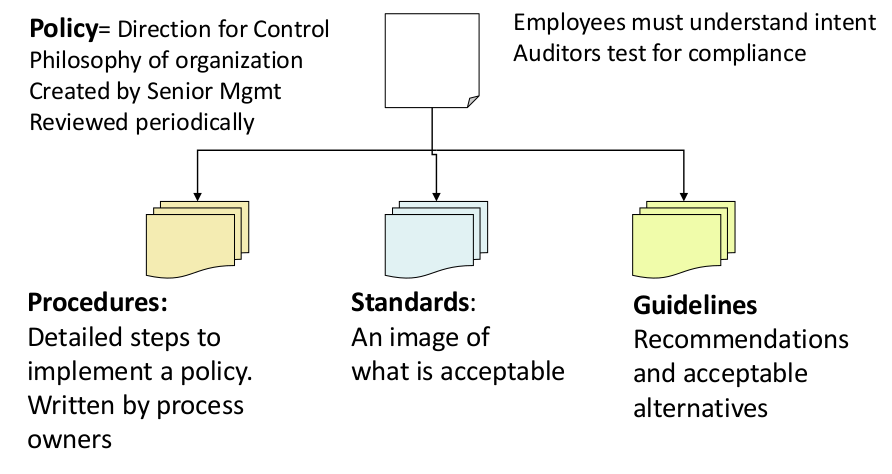
\includegraphics[scale=0.4]{res/img/documentation_policy}
        \end{center}
        \caption{Policy per la documentazione.}
\end{figure}

\subsubsection{Esempi di policy}

I \textbf{rischi} dovrebbero essere gestiti utilizzando dei controlli e delle 
contromisure appropriate per raggiungere dei livelli accettabili a dei costi 
accettabili. Il \textbf{monitoraggio} e le \textbf{metriche} dovrebbero essere 
implementate, gestite e mantenute per fornire una certezza continua che tutte 
le policy sulla sicurezza siano rispettate e i controlli oggettivi siano 
riscontrati. Le \textbf{capacità di risposta ad incidenti} sono implementate e 
gestite sufficientemente per garantire che gli incidenti non affliggano 
materialmente la capacità dell'organizzazione di continuare le proprie 
operazioni. 
La \textbf{business continuity} e il \textbf{recovery plan} dovrebbero essere 
sviluppate, mantenute e testate in modo che assicurino la capacità 
dell'organizzazione di proseguire con le proprie attività sotto tutte le 
condizioni.

Nota: una cattiva \textit{policy} fa riferimento alla tecnologia. Le 
\textit{policy} sono solamente linee guida.

\subsubsection{Policy, procedure e standard}

\paragraph*{Obiettivo di una policy:} descrive \textit{cosa} deve essere 
soddisfatto.

\paragraph*{Controllo della policy:} tecniche per raggiungere l'obiettivo, 
suddivise in
\begin{itemize}
  \item \textbf{Procedure:} definiscono come la policy deve essere perseguita;
  \item \textbf{Standard:} regola, metrica o vincolo specifico che implementa 
  la policy.
\end{itemize}

\subsubsection{Definizioni della qualità}

\paragraph*{Quality assurance:} assicurarsi che tutto lo staff stia seguendo i 
processi della qualità definiti.

\paragraph*{Controllo della qualità:} condurre test per validare che il 
software è privo di difetti e corrisponde alle aspettative dell'utente.

\subsection{Livello 4 - Metriche}

Esistono degli obiettivi misurabili per la qualità della sicurezza, le misure 
sono correlate agli obiettivi del business dell'organizzazione. Le 
funzionalità comuni includono: stabilire degli obiettivi misurabili di qualità 
e una gestione oggettiva delle performance (SLA).
È tutto scritto e documentato: sono presenti politiche, 
procedure, standard e linee guida.

\subsubsection{Metriche}

Le metriche permettono ad auditor differenti di attestare che i programmi per 
la sicurezza vengono attuati. Monitorare il raggiungimento di controlli 
oggettivi è più importante che perfezionare le procedure di sicurezza.

Senza metriche quantitative si lascia spazio alla soggettività.

\begin{figure}[h!]
        \begin{center}
                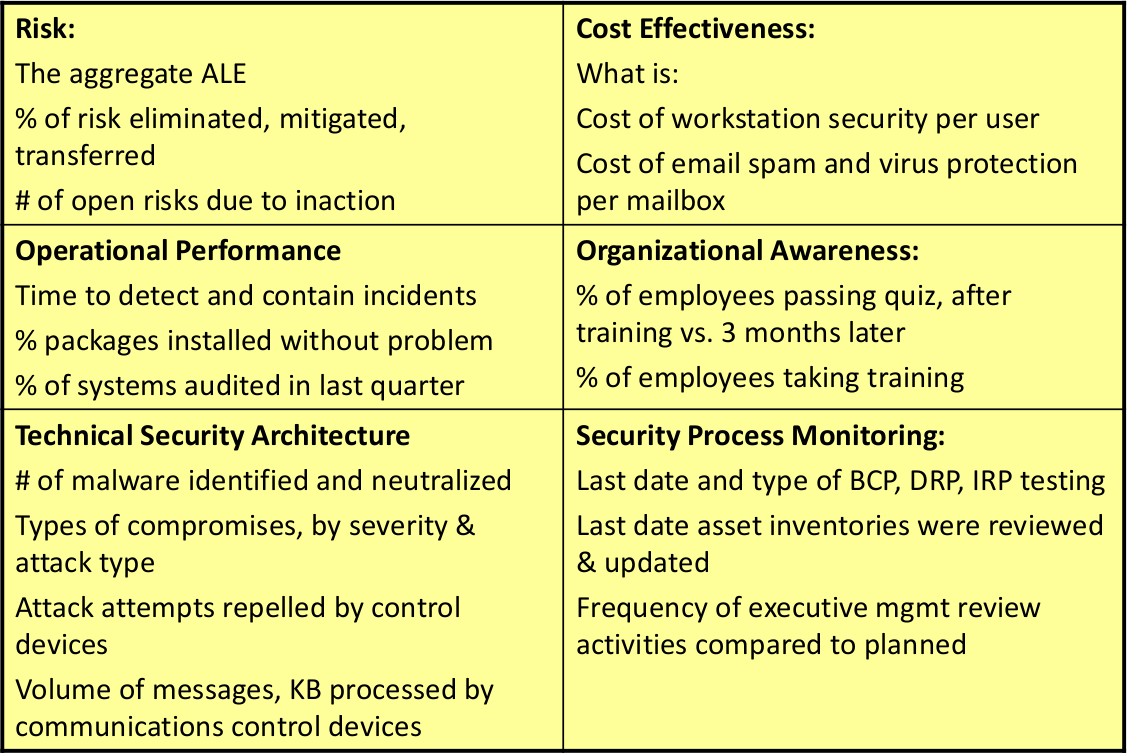
\includegraphics[scale=1.5]{res/img/metriche}
        \end{center}
        \caption{Esempi di metriche per un'azienda.}    
\end{figure}

\paragraph*{Metriche operazionali}

Le metriche di tipo operazionale includono metriche su come eseguire 
un corretto \textit{patching} dei sistemi.

Confrontare le metriche con quelle di altre aziende permette di capire quanto 
siamo un possibile \textit{target} per gli attaccanti.

\paragraph*{Metriche di tipo strategico}

Sono i piani legati al rischio, come il \textit{disaster recovery}.
Il rapporto di audit è una metrica importantissima perché fa capire come 
lavora l'azienda e l'auditor.

\paragraph*{Compliance interna}

La conformità (\textit{compliance}) assicura la conformità con le policy 
organizzative. Compliance e errore interno sono dati importanti perché 
fanno capire all'azienda quanto è allineata con gli obiettivi strategici che 
si è prefissata.


\subsection{Livello 5 - Miglioramento continuo}

Il miglioramento continuo parte dalle misure e dagli eventi sulla sicurezza.
Vengono valutate nuove tecnologie e nuovi processi. Le funzionalità comuni 
includono: miglioramento delle capacità organizzative e della efficacia dei 
processi (ROI).

Prima avere un cambio tecnologico di fondo è raro, oggi avviene ogni 3 anni. 
Chi prende la tecnologia e la incorpora si prende la fetta di mercato.

Le grandi società fanno \textit{scouting} di nuove tecnologie. Il vantaggio di 
essere un'azienda piccola è che si può essere aggressivi e investire, aiutando 
il movimento economico. Questo ci dice che aziende come Google non ci 
saranno per sempre. Non si è ancora capito a dove possa portare il cambiamento
tecnologico. Un'altra area importante è l'intelligenza artificiale legata 
alla sicurezza.


\section{COBIT \& COSO}

\textbf{COSO} è un modello strategico per la governance dell'azienda. 
Purtroppo è troppo complesso per un'azienda di dimensioni medio grandi e 
quindi è caduto in disuso.\\
\newline
\textbf{COBIT} è un insieme di raccomandazioni finalizzate alla \textit{
governance} 
del sistema IT a livello operativo.
COBIT deriva da COSO ed è allineato con esso. In particolare il grafico in 
Figura~\ref{fig:cobit:coso:relazione} mostra la relazione tra COSO e COBIT
\footnote{Esistono manuali gratuiti 
riguardo COBIT, che spaziano dal livello \textit{entry} fino a quelli più 
avanzati. Questi manuali sono consigliati a chi vuole approcciarsi a questo 
ambiente lavorativo. Al seguente link per esempio è possibile trovare un 
manuale riguardo COBIT4:  \url{https://www.isaca.org/Italian/Documents/
CobiT-41-Italian.pdf}}.
\begin{figure}[h!]
        \begin{center}
                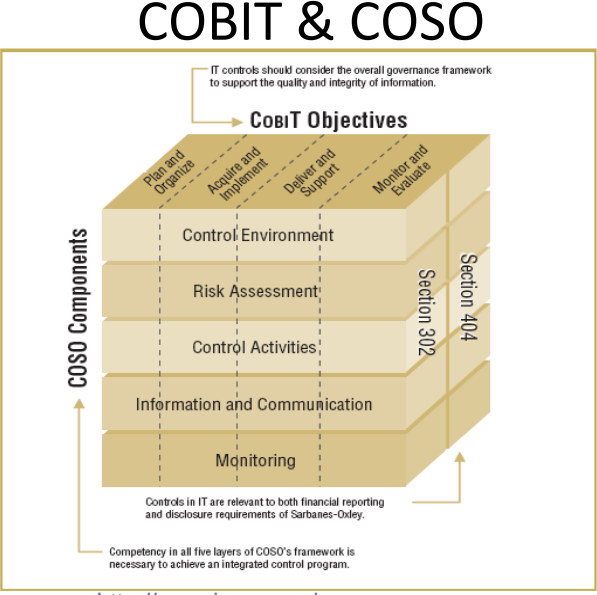
\includegraphics[scale=2.0]{res/img/cobit_coso_cube}
        \end{center}
        \caption{Grafico che mostra la relazione tra COBIT e COSO.}
        \label{fig:cobit:coso:relazione}
\end{figure}

\subsection{COBIT}
\label{COBIT}

\begin{enumerate}
  \item Pianificazione e organizzazione;
  \item Acquisizione e implementazione;
  \item Consegna e supporto;
  \item Monitoring
\end{enumerate}

\subsubsection{Pianificazione e organizzazione}

In un'azienda IT è importante definire un piano strategico per l'IT. Si è 
passati dall'avere un insieme di applicazioni centralizzate ad architetture 
distribuite \textit{cloud}-centriche. Chi ha previsto queste innovazioni ieri, 
oggi sta guadagnando molto.

L'\textit{information architecture} si focalizza su come viene distribuita 
l'informazione, su come viene distribuito il dato e su come aggiunge 
informazione al dato.

La tendenza tecnologica è quella di andare verso un IT decentralizzato. La 
manutenzione è importante ed è quindi altrettanto importante capire che una 
rivisitazione dei costi IT non è possibile che venga eseguita a costo 0. I 
processi messi in piedi sono molti importanti. La comunicazione è fondamentale 
ed è un difetto di informatici e ingegneri. La non-comunicazione fa appassire 
le idee\footnote{Perla del professore: \textbf{una buona idea comunicata bene 
ottiene molto di più di un'idea eccellente comunicata male.}} e questo viene 
aggravato dall'inerzia che ha una grande azienda, in quanto un gran numero di 
persone si muovono lentamente tra loro.

Anche le risorse IT sono importanti: non serve più solo prendere ``quello 
bravo'', ma è importante avere un piano di \textit{retention}, ovvero capire 
come mantenere i dipendenti (soprattutto le persone chiave) all'interno 
dell'azienda. Questo andrebbe fatto anche nelle aziende piccole (20-30 
dipendenti)\footnote{Il professore consiglia di andare a vedere il PMI: 
\textit{Project Management Institute}, che spiega come gestire vari progetti.}.

\begin{itemize}
\item PO1: definire un piano IT strategico;
\item PO2: definire l'architettura dell'informazione;
\item PO3: determinare la direzione tecnologica;
\item PO4: definire i processi IT, l'organizzazione e le relazioni;
\item PO5: gestire gli investimenti nell'IT;
\item PO6: comunicare al management direzione e obiettivi;
\item PO7: gestire le risorse umane dell'IT;
\item PO8: gestire la qualità;
\item PO9: valutare e gestire i rischi IT; 
\item PO10: gestire i progetti.

\end{itemize}

\subsubsection{Acquisizione e implementazione}

\begin{itemize}
\item AI1: identificare soluzioni automatizzate;
\item AI2: acquisire e mantenere le applicazioni software;
\item AI3: acquisire e mantenere l'infrastruttura tecnologica;
\item AI4: abilitare operazioni e utilizzo;
\item AI5: procurare le risorse IT;
\item AI6: gestire i cambiamenti;
\item AI7: installare e accreditare soluzioni e cambiamenti.
\end{itemize}

\subsubsection{Consegna e supporto}

Quando si hanno servizi di diverse parti i SLA\footnote{Service Learning 
Agreement} sono fondamentali. Gestione e capacità sono concetti diversi.
Quando si ha settato un'organizzazione il limite estremo è la capacità 
ottimale (è quando tutti lavorano al 100\%, che è impossibile). Da qui bisogna 
capire dove si è e quanto ce n'è, e questo viene detto \textit{capacity}. 
Siccome è molto difficile per aziende grosse si guardano gli indicatori 
finanziari.